
\chapter{Conclusion} \label{chp:conclusion}


This thesis presents a novel compiler optimisation based on function merging to reduce code size.
The function merging optimisation consists in combining multiple functions with similarity into a single function, in order to reuse code, removing redundancies, and reducing code size.

%Chapter~\ref{chp:cgo19} describes our novel approach, based on sequence alignment, for merging any two functions.
%We also describe how this function merging technique can be integrated with an optimisation strategy.
%In order to find profitable merged functions, we propose a fingerprint-based ranking mechanism and a profitability cost %model.
%Chapter~\ref{chp:pldi20} 

%describes how our function merging technique can be combined with a optimisation strategy in order to search for profitable functions to merge, which includes a profitability cost model and a ranking of candidate functions.

%This chapter is structured as follows:
%Section~\ref{sec:conclusion:contribution} summarises the main contributions of this thesis,
%%%%Section 7.2 presents a critical analysis of this work,
%Section~\ref{sec:conclusion:futurework} describes future research directions,
%and finally Section~\ref{sec:conclusion:summary}  provides concluding remarks.

\section{Contribution} \label{sec:conclusion:contribution}

\subsection{Function Merging Optimisation}

Chapter~\ref{chp:cgo19} describes a novel function merging optimisation.
Our function merging technique is the first capable of merging any two functions.
In order to achieve that, our technique uses sequence alignment algorithms, from bioinformatics, to identify regions of similarity and difference between two functions.
The sequence alignment algorithm produces this similarity information by searching for the best alignment between sequences, given a penalty system. 
The resulting aligned sequence is then used to generate a merged function that can replace both input functions.

Since we are able to merge arbitrary pairs of functions, we also need to identify which pairs of functions can be profitably merged, reducing code size.
First, we use a profitability cost model that estimates the binary size of the input functions and the merged function.
Two input functions can be profitably merged if replacing them by a merged function results in an overall smaller code.
Then we integrate our function merging technique with a search strategy.

Trying to merge every pair of functions in order to identify the most profitable ones is prohibitive.
Besides the quadratic search itself, merging two functions involve a sequence alignment, which is quadratic on the size of the functions.
Since an exhaustive search is infeasible, we need a better search strategy.
First, we pre-compute the fingerprint, which is a fixed-size representation, of every function in the program.
These fingerprints can be efficiently compared in constant time.
For each function, the search strategy consists in ranking all other candidate functions based on a fingerprint similarity.
Finally, the proposed optimisation will attempt to merge only the top ranked candidate functions.

Our optimization is able to reduce code size by up to 25\%, with an overall average of about 6\%, while introducing an average compilation-time overhead of only 15\%.
Compared to prior techniques, which contain many limitations on which functions they can merge, our approach is able to outperform them by more than 2.4$\times$ on code size reduction.
Moreover, coupled with profiling information, our optimization introduces no statistically significant impact on performance.

\subsection{Effective Code Generator for the SSA Form}

In order to simplify its code generator, the technique proposed in Chapter~\ref{chp:cgo19} replaced all phi-nodes with memory operations by first applying register demotion.
This tends to almost double the function size, increasing compilation time and hindering function merging, as it expects that applying register promotion to the merged function will reverse the negative effect of the earlier register demotion.
This is often not possible because function merging can add complexity to the memory operations, resulting in unnecessarily larger merged functions.

Chapter~\ref{chp:pldi20} describes a novel approach for merging functions which is capable of effectively handling the SSA form.
The proposed approach, called SalSSA, achieves this with a new code generator.
Instead of translating the aligned sequences directly into a merged function, SalSSA generates code from the input control-flow graphs, using the alignment only to specify pairs of matching labels and instructions.
The generator then produces code top-down, starting with the control flow graph of the merged function, then populating with instructions, arguments and labels, and finally with phi-nodes which maintain the correct flow of data.

Chapter~\ref{chp:pldi20} also introduces a novel phi-node coalescing optimisation which is integrated with function merging in order to produce fewer phi-nodes and selections in the merged functions.
This optimisation pairs disjoint values coming from each one of the input functions so that they can share the same phi-nodes.


\subsection{}


\section{Future Work} \label{sec:conclusion:futurework}

For future work, we plan to focus on improving the ranking mechanism to reduce compilation time.
In order to avoid code size degradation, we also plan to improve the compiler's built-in static cost model for code size estimation.
We also plan to work on the linearisation of the candidate functions, allowing instruction reordering to maximize the number of matches between the functions.
Finally, we also plan to incorporate instruction reordering into function merging to maximize the number of matches between the functions regardless of the original code layout.
One can also investigate the application of phi-node coalescing outside function merging.
We envisage further improvements can be achieved by integrating the function-merging optimization to a summary-based  link-time optimization framework, such as ThinLTO in LLVM.
As a future work, we can also analyze the interaction between function merging and other optimizations such as inlining, outlining, and code splitting.

\subsection{Better Code Generator}

%FMSA's code generator is responsible for producing the actual merged functions from the aligned sequences.
%In its original version, FMSA has many artificial limitations in order to simplify its code generator.
%Preliminary results show that the code generator can be significantly improved, enabling far more code compression while reducing compilation time overhead.
%For this project, we plan to develop a new code generator that is capable of appropriately handling $\phi$-nodes, variable length arguments, calling convention, and exploiting target specific instructions to better compress code.
%There are still many opportunities to optimize operand selection and branch instructions that result from merging code. 

In order to better compress code, one can improve the code generator, optimising the parameters used as function identifiers based on calling conventions, exploit target specific instructions, and optimize operand selection and branch instructions that result from merging code.
There are also many missing features in the code generator that are important for its application in the industry.
For example, a new code generator could also be able to appropriately handle variable length arguments, and debug information.
When merging functions, having an optimised code generator is as important as optimally identifying which instructions to merge.
%In the industry, it is also crucial that we appropriately handle debug information when generating code. %link with: \phi$-nodes, variable length arguments
%Appropriately generating code with debug information is crucial for its application in the industry.

\subsection{Handling Code Reordering}

All existing function merging techniques rely on the order in which instructions appear inside the basic blocks and their arrangement,
failing to profitably merge equivalent functions when confronted even with the smallest variations on the ordering of instructions and basic blocks.
Figure~\ref{fig:code-reordering} shows an example of two functions that all existing techniques fail to merge even though they are obviously identical.
Our current technique produces the merged function shown in Figure~\ref{fig:merged-code-reordering}, which is considered unprofitable as it is unable to reduce code size.
Note that all indexing computation is duplicated, including the increment operation, resulting in a merged function that is unnecessarily bigger than the two original functions together.
We need more powerful graph, rather than sequence, alignment techniques to better identify and merge differently ordered but semantically equivalent code.

\begin{figure}[h]
 \centering
 \begin{subfigure}{.75\textwidth}
         \centering
         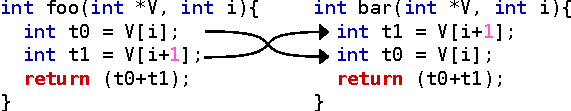
\includegraphics[scale=1]{src/conclusion/figs/motivation-1-code.pdf}
        %  \vspace{1ex}
         \caption{Two equivalent functions.}
         \label{fig:code-reordering}
 \end{subfigure}
 \\
 \begin{subfigure}{.75\textwidth}
         \centering
         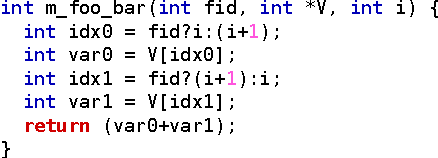
\includegraphics[scale=1]{src/conclusion/figs/motivation-1-merged-code.pdf}
         \caption{Merged function currently produced by FMSA.}
         \label{fig:merged-code-reordering}
 \end{subfigure}
    \vspace{-2ex}
    \caption{Example of how even trivial reordering is poorly handled by the existing solutions.}
    \label{fig:code-reordering-example}
\end{figure}

\subsection{Merging Across All Scopes}

Existing techniques are limited to one particular scope.
While function merging is applied only to whole functions,
function outlining is commonly applied at the basic block level.
%In one end we have an optimization such as the function outlining which is capable of merging or extracting equivalent basic blocks, in the other end we have function merging capable of merging whole functions.
However, equivalent code can be found within or across functions, which themselves may reside in the same source file or be spread across multiple source files.
Therefore, we need to develop a novel unified optimization capable of merging semantically equivalent code that can span anything between a single basic block up to a whole function.
This unification has the extra benefit of also addressing the phase ordering problem by coordinating the merge operations on different scopes.

\subsection{Scaling for Large Programs}

Although our optimisation achieves very good results in terms of code compression, it is still unable to handle large programs in a real scenario.
Its time complexity and memory usage requirements would prevent it from optimizing large programs such as web browsers, Clang/LLVM, and operating systems, as these programs tend to have many functions with several thousands of instructions.
Link-time optimization (LTO) makes this matter even worse by optimizing the code after the whole program has been linked into a single module, imposing a huge pressure on memory usage and compilation time.

%In this project, we will investigate this scalability issue.
%We plan to perform link-time optimization in an incremental fashion, such as using ThinLTO, which operates on individual translation units, reducing memory usage while also making it suitable for parallel and distributed compilation.
The optimization of different translation units can be distributed across different machines and merge operations locally performed in parallel.
In order for this to work, an important challenge that needs to be addressed concerns ranking and merging functions that reside in different translation units.
However, this is essential to enable the use of LTO on real programs while keeping the memory usage and compilation time acceptable.

\subsection{Powered by Deep Learning}

One can investigate the use of deep learning to align two functions and better identifying what can be merged.
Sequence alignment focusses only on maximizing the number of merged instructions,
without necessarily minimizing the number of operand selections or branches.
A smarter approach that understands how instructions interact with each other would be
very beneficial.

\subsection{Avoiding Performance Overheads}

For many real applications, it is desirable to achieve a good balance between code size and performance.
Preliminary results show that performance degradation can be completely avoided by using profiling to
guide the merging decisions.
One can avoid adding branches inside hot execution paths, therefore avoiding performance penalties.
Although hot code can be merged, it is important to minimize unnecessary branches when merging hot code.
We will develop a profile-guided optimization that automatically identify the best trade-off between code-size and performance.

\subsection{Less Memory Usage by JIT}

Ahead-of-time and just-in-time (JIT) compilation have completely different requirements.
Function merging can be used to reduce the amount of memory used by programs running on a JIT environment.
However, our solution must be adapted to the requirements that are specific to a JIT environment, as JIT compilers have the extra challenge of having to optimize the code as fast as possible.
This would require the development of completely new algorithms for ranking and aligning functions that are suitable for this application domain.
Another possibility is to exploit the fact multiple programs may be simultaneously running on the same JIT environment and merge code across different programs, reducing the overall memory usage.

%\section{Summary} \label{sec:conclusion:summary}